\documentclass[11pt,twoside]{template-ubi/Styling}

\setmainfont{Georgia}

\usepackage{listings}
\lstset{
	language=C++,                % choose the language of the code
	basicstyle=\footnotesize,       % the size of the fonts that are used for the code
	numbers=left,                   % where to put the line-numbers
	numberstyle=\footnotesize,      % the size of the fonts that are used for the line-numbers
	stepnumber=1,                   % the step between two line-numbers. If it is 1 each line will be numbered
	numbersep=5pt,                  % how far the line-numbers are from the code
	backgroundcolor=\color{white},  % choose the background color. You must add \usepackage{color}
	showspaces=false,               % show spaces adding particular underscores
	showstringspaces=false,         % underline spaces within strings
	showtabs=false,                 % show tabs within strings adding particular underscores
	frame=single,           % adds a frame around the code
	tabsize=2,          % sets default tabsize to 2 spaces
	captionpos=b,           % sets the caption-position to bottom
	breaklines=true,        % sets automatic line breaking
	breakatwhitespace=false,    % sets if automatic breaks should only happen at whitespace
	escapeinside={\%*}{*)}          % if you want to add a comment within your code
}

% Comment this line if you are writing your thesis in English
% \portugues

%%Para gerar índice remissivo (que será inserido no documento com o comando \printindex)
\makeindex

\thesistitle{Thesis Title}
% Se existir um sub-título, descomente a linha abaixo e 
%\thesissubtitle{Sub-título da Tese}

%Nome da faculdade
\facultyname{Engenharia}

% Ciclo de estudos (1º, 2º ou 3º)
\studiescyclenumber{3\textsuperscript{o}}

\thesisauthors{Your name here}
\thesistype{Tese para obtenção do Grau de Doutor em}
\thesislocalanddate{Maio de 2021.}

\thesissupervisors{
	Orientador: Prof. Doutor Name of your Surpervisor\\
	%Co-orientador: Prof. Doutor Name of your Co-Surpervisor\\
}

% Name of your course
\thesiscourse{Engenharia Informática}

% O comando seguinte insere o nome da tese no cabeçalho das páginas (comentar se não for pretendido)
% (Pode ser o título abreviado)
% \cabecalho{\thesistitlestr}

\begin{document}

\thesisfunding{
	Inserir informações sobre financiamento da tese. (Opcional: se não desejar incluir, todo o comando deve ser apagado)\\
}

% Se desejar colocar o conteúdo de uma secção em um ficheiro tex separado,
% tal ficheiro pode ser incluído usando o comando \input{Nome do ficheiro criado}.
% Exemplo: \thesisdedication{\input{nome-do-ficheiro-contendo-a-dedicatoria}}
% Isto resulta para todas as seções abaixo.
\thesisdedication{
	Inserir dedicatória. (Opcional: se não desejar incluir, todo o comando deve ser apagado)\\
}

\thesisthanks{
	Agradecer a quem de direito. (Opcional: se não desejar incluir, todo o comando deve ser apagado)
}

\thesisforewords{
	Prefácio. (Opcional: se não desejar incluir, todo o comando deve ser apagado)
}

% Abstract in Portuguese
\thesisresumo{
	Resumo do trabalho em português, seguida das palavras-chave.
}{Suas, palavras, chaves, separadas, por, vírgula}


% Expanded Abstract in Portuguese
\thesisresumoalargado{
	Resumo alargado deve ser escrito em português e é usado unicamente para 
	teses escritas em língua estrangeira.
	Se não for este o caso, todo o comando deve ser apagado.
} 	

\thesisabstract{
	Abstract in English, followed by keywords.
}{Your, key, words, separated, by, comma}	

\tableofcontents   % Índice
\listoffigures     % Lista de Figuras    (Opcional)
\listoftables      % Lista de Tabelas    (Opcional)
\listofalgorithms  % Lista de Algoritmos (Opcional)
\thesisacronyms{\begin{tabularx}{\linewidth}{c p{0.5cm} Y}
 	UBI & & Universidade da Beira Interior\cr
 	MPSOCD & & Multi-objective Particle Swarm Optimization Crowding Distance
\end{tabularx}
}  % Lista de Acrónimos  (Opcional)

\mainmatter % inicia páginas em números arábicos a partir do 1
\acresetall

% Os capítulos são inseridos a partir daqui 
\chapter{Introduction} \label{chap:int}

\section{Thesis Focus and Scope} \label{sec:focus}

IoT \cite{friis} basically refers to ....\\
%\ac{IoT} basically refers to ....\\
\chapter{State-of-the-Art} \label{chap:state_of_the_art}

This chapter describes ....
\chapter{Basic Concepts 123} \label{chap:basic_concepts_123}

This chapter prepares the ....
\chapter{The ABC} \label{chap:the_abc}

This chapter will ....

\chapter{The XYZ} \label{chap:the_xyz}

This chapter ....


\chapter{Samples} \label{chap:ex}

Neste capítulo exemplifica-se como inserir alguns ambientes (enumeração, tabela, figura).

\begin{enumerate}
	\item Resistência\index{Resistência} -- É um elemento passivo que dissipa energia sob a forma térmica;
	\item Condensador\index{Condensador} -- É um elemento que armazena energia num campo eléctrico.
\end{enumerate}

A Tabela \ref{tab:001} contém o código de cores das resistências\footnote{Apenas código para primeira e segunda cor. Não inclui tolerância nem factor multiplicativo. Apenas código para primeira e segunda cor. Não inclui tolerância nem factor multiplicativo. Apenas código para primeira e segunda cor. Não inclui tolerância nem factor multiplicativo}.

\begin{table}[h!]
\caption{Correspondência entre as cores das riscas das resistências e o seu valor óhmico.}
	\centering
		\begin{tabular}{|c|c|}
		\hline
			\textbf{Cor} & \textbf{Valor} \cr
			\hline
			Preto & 0 \cr
			\hline
			Castanho & 1 \cr
			\hline
			Vermelho & 2 \cr
			\hline
			Laranja & 3 \cr
			\hline
			Amarelo & 4 \cr
			\hline
			Verde & 5 \cr
			\hline
			Azul & 6 \cr
			\hline
			Violeta & 7 \cr
			\hline
			Cinzento & 8 \cr
			\hline
			Branco & 9 \cr
			\hline
		\end{tabular}
	\label{tab:001}
\end{table}

Considere-se o circuito da Figura \ref{fig:ohm}.

\begin{figure}[h]
	\centering
		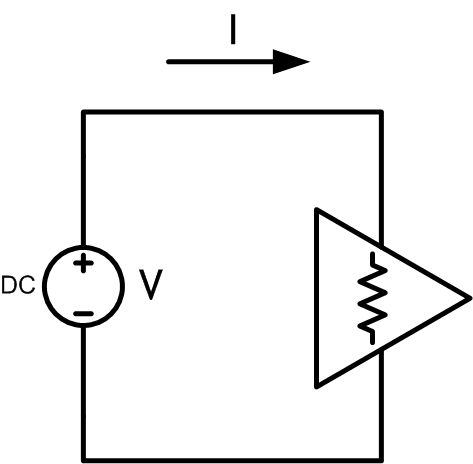
\includegraphics[height=3cm]{leiOhm}
	\caption{Circuito básico com uma fonte de tensão contínua (V) e uma resistência atravessada por uma corrente I.}
	\label{fig:ohm}
\end{figure}

Pode-se calcular a corrente que circula na resistência através da equação \ref{for:ohm}, denominada de Lei de Ohm\index{Lei de Ohm}.


\begin{equation}\label{for:ohm}
	I=\frac{V}{R}
\end{equation}

O texto pode vir em \textbf{negrito} ou em \textit{itálico} ou \textbf{\textit{ambos}}.

O Algoritmo \ref{alg1} serve de base para o nosso sistema de controlo do semáforo da igreja.
\begin{algorithm}
	\caption{Pseudo código para o semáforo.}
	\label{alg1}
	\begin{algorithmic}
		\STATE Início
		\FOR{todas as luzes}
			\IF{sem corrente}
				\STATE informar de avaria
			\ELSE
				\STATE luz ok
			\ENDIF 
		\ENDFOR
		
		\LOOP
			\STATE accionar verde no semáforo principal
			\STATE aguardar por sinal dos sensores de posição
			\IF{carro no sensor}
				\STATE mudar para vermelho semáforo principal
			\ENDIF
		\ENDLOOP
		\STATE \textbf{until} interruptor de manutenção activado
	\end{algorithmic}
\end{algorithm}


\chapter{Conclusions and Future Work} \label{chap:conclusion}

Your conclusion here.
 
 

% Fim da inserção dos capítulos

% Bibliografia
% Primeiro parâmetro é o estilo e o segundo o arquivo bib
\thesisbibliography{template-ubi/BiblioStyle}{bibliography}

% Exemplo de uso de outro estilo bibliográfico. Define ser definido apenas um estilo 
%\thesisbibliography{template-ubi/IEEEtran}{bibliografia}

\appendix{\chapter{Appendix} \label{chap:appendix}

Nam placerat ullamcorper ante non venenatis. Phasellus et ipsum at lorem rhoncus euismod. Phasellus in risus elit, sed mollis dolor. Aenean non ligula ut metus porta laoreet. Duis mi quam, sollicitudin non posuere eu, facilisis vestibulum purus. Cras eget odio et diam imperdiet consectetur eu vel libero. Cras in dapibus felis. Praesent sed nunc neque. Donec lobortis venenatis pretium. Praesent quis lorem ipsum, id mattis ante. 

\section{Datasheets dos componentes utilizados}

Lorem ipsum dolor sit amet, consectetur adipiscing elit. Praesent at magna viverra neque bibendum pellentesque. Morbi ullamcorper auctor turpis vitae mollis. Fusce elementum mauris eu magna tristique vel aliquet erat iaculis. Donec sed augue mi. Aenean commodo lorem ac nulla iaculis rhoncus. Mauris facilisis, ante in molestie bibendum, lorem augue vehicula metus, ac auctor turpis quam nec purus. Nam malesuada accumsan neque, quis vulputate nibh dapibus vitae. Vestibulum eu arcu ut est posuere malesuada. Donec aliquet, mauris vel viverra bibendum, risus sem fringilla orci, placerat laoreet felis velit ac justo. Mauris sit amet sollicitudin magna. Sed commodo enim sed nibh consectetur cursus. Duis turpis lacus, semper non facilisis eu, semper eu lacus. Donec vel urna urna, eget gravida magna.} % Anexos (Opcional)
\thesisglossary{\begin{tabularx}{\linewidth}{l p{0.5cm} Y}
	\LaTeX & & Conjunto de macros para o processador de textos \TeX, utilizado amplamente para a produção de textos matemáticos e científicos devido à sua alta qualidade tipográfica.\cr
\end{tabularx}}  % Glossário (Opcional)

\printindex % Inserir índice remissivo (Opcional)

\end{document}
